\section{Definition}

\subsection{Project Overview}

In this project, a mail-order sales company in Germany is interested in identifying segments of the general population to target with their marketing, to grow their customer base. Demographics information is available for both the general population as well as for prior customers of the company. We use this information to build a model of the customer base of the company. The target dataset contains demographic information for targets of a mailout marketing campaign. The objective is to identify which individuals are most likely to respond to the campaign and become customers of the mail-order company.

The data has been provided by Bertelsmann Arvato Analytics and consists of four data files: 

\begin{itemize}
\item \emph{Udacity\textunderscore AZDIAS\textunderscore 052018.csv}: Demographics data for the general population of Germany; 891 211 persons (rows) x 366 features (columns).
\item \emph{Udacity\textunderscore CUSTOMERS\textunderscore 052018.csv}: Demographics data for customers of a mail-order company; 191 652 persons (rows) x 369 features (columns).
\item \emph{Udacity\textunderscore MAILOUT\textunderscore 052018\textunderscore TRAIN.csv}: Demographics data for individuals who were targets of a marketing campaign; 42 982 persons (rows) x 367 (columns).
\item \emph{Udacity\textunderscore MAILOUT\textunderscore 052018\textunderscore TEST.csv}: Demographics data for individuals who were targets of a marketing campaign; 42 833 persons (rows) x 366 (columns).
\end{itemize}
The "CUSTOMERS" file contains three extra columns ('CUSTOMER\textunderscore GROUP', 'ONLINE\textunderscore PURCHASE', and 'PRODUCT\textunderscore GROUP'), which provide broad information about the customers depicted in the file. Each row of the demographics files represents a single person, but also includes information outside of individuals, including information about their household, building, and neighborhood.

\subsection{Problem Statement}

The goal is to identify segments of the population that form the core customer base for the company. These segments can then be used to direct marketing campaigns towards audiences that have the highest expected rate of returns.

The information from the first two files is used to figure out how customers ("CUSTOMERS") are similar to or differ from the general population at large ("AZDIAS"), then use this analysis to make predictions on the other two files ("MAILOUT"), predicting which recipients are most likely to become a customer for the mail-order company.

The original "MAILOUT" file included one additional column, "RESPONSE," which indicated whether or not each recipient became a customer of the company. For the "TRAIN" subset, this column is present, but in the "TEST" subset it has been removed; it is against that withheld column that we will asses the final predictions. The higher the score obtained, the better the model is at predicting customers.

\subsection{Metrics}

We are dealing with an imbalanced classification problem, and we consider using metrics beyond accuracy such as recall, precision, and AUROC.

The evaluation metric chosen for this project is AUC for the ROC curve (see figure \ref{fig:auroc}), relative to the detection of customers from the mail campaign. A ROC, or receiver operating characteristic, is a graphic used to plot the true positive rate (TPR, the proportion of actual customers that are labeled as so) against the false positive rate (FPR, the proportion of non-customers labeled as customers).

The line plotted on these axes depicts the performance of an algorithm as we sweep across the entire output value range. We start by accepting no individuals as customers (thus giving a 0.0 TPR and FPR) then gradually increase the threshold for accepting customers until all individuals are accepted (thus giving a 1.0 TPR and FPR). The AUC, or area under the curve, summarizes the performance of the model. If a model does not discriminate between classes at all, its curve should be approximately a diagonal line from (0, 0) to (1, 1), earning a score of 0.5. A model that identifies most of the customers first, before starting to make errors, has its curve start with a steep upward slope towards the upper-left corner before making a shallow slope towards the upper-right. The maximum score possible is 1.0 if all customers are perfectly captured by the model first.

\begin{figure}[h]
\centering
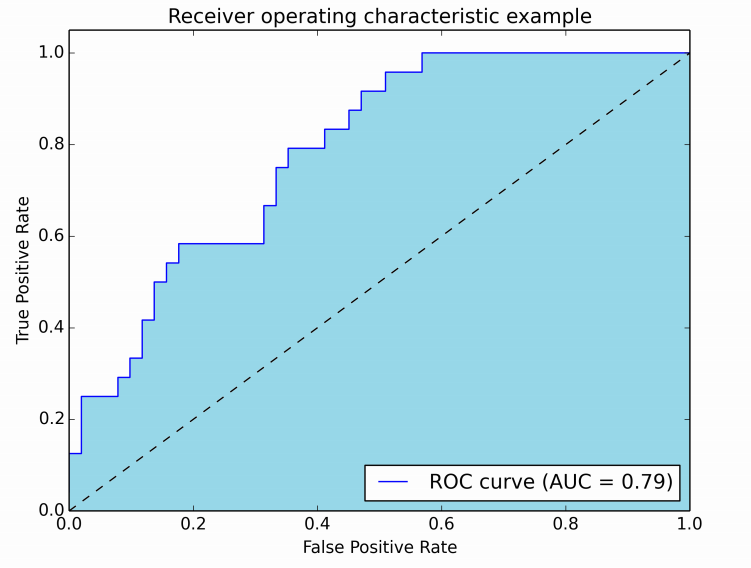
\includegraphics[width=0.5\textwidth]{roc_curve.png}
\caption{Example of how AUROC looks graphically}
\label{fig:auroc}
\end{figure}